\documentclass[10pt,a4paper]{report}
%\usepackage[latin1]{inputenc}
\usepackage[utf8]{inputenc}
\usepackage{amsmath}
\usepackage{amsfonts}
\usepackage{amssymb}
\usepackage{graphicx}
\usepackage{multicol}
\usepackage{tabularx}
\usepackage{tikz}
\usetikzlibrary{arrows,shapes,automata,petri,positioning,calc}
\usepackage{hyperref}
\usepackage{tikz}
\usetikzlibrary{matrix,calc}
\usepackage[margin=0.5in]{geometry}
% ---- power functions -----% 
\newcommand{\myvec}[1]{\ensuremath{\begin{pmatrix}#1\end{pmatrix}}}
\let\vec\mathbf

\providecommand{\norm}[1]{\left\lVert#1\right\rVert}
\providecommand{\abs}[1]{\left\vert#1\right\vert}
\let\vec\mathbf

\newcommand{\mydet}[1]{\ensuremath{\begin{vmatrix}#1\end{vmatrix}}}
\providecommand{\brak}[1]{\ensuremath{\left(#1\right)}}
\providecommand{\lbrak}[1]{\ensuremath{\left(#1\right.}}
\providecommand{\rbrak}[1]{\ensuremath{\left.#1\right)}}
\providecommand{\sbrak}[1]{\ensuremath{{}\left[#1\right]}}
%-------end power functions----%
\newenvironment{Figure}
  {\par\medskip\noindent\minipage{\linewidth}}
  {\endminipage\par\medskip}
\begin{document}
%--------------------logo figure-------------------------%
\begin{figure*}[!tbp]
  \centering
  \begin{minipage}[b]{0.4\textwidth}
    
\includegraphics[scale=0.05]{iitlogo.jpg} 
  \end{minipage}
  \hfill
  \vspace{5mm}\begin{minipage}[b]{0.4\textwidth}
\raggedleft  
\includegraphics[scale=0.05]{nrc.png}  \

  \end{minipage}\vspace{0.2cm}
\end{figure*}
%--------------------name & rollno-----------------------
\raggedright \textbf{Name}:\hspace{1mm} Cheenepalli Chandana\hspace{2cm} \Large \textbf{Conic Assignment}\hspace{2.5cm} % 
\normalsize \textbf{Roll No.} :\hspace{1mm} FWC22062\vspace{1cm}
\begin{multicols}{2}

%----------------problem statement--------------%
\raggedright \textbf{Problem Statement:}\vspace{2mm}
\raggedright \\Find the area enclosed by the parabola $4y=3x^2 $ and the line $2y=3x+12$\\
\vspace{5mm}
%-----------------------------solution---------------------------
\raggedright \textbf{SOLUTION}:\vspace{2mm}\\

%---------given----------------%
\raggedright \textbf{Given}:\vspace{2mm}\\
Equation of parabola is \\\vspace{1mm}
\begin{align}
4y=3x^2
\end{align}
Equation of line is \\ \vspace{1mm}
\begin{align}
2y=3x+12
\end{align}
%-------------To find ------------------%
\textbf{To Find }\vspace{2mm}\\
To find the intersection points and area enclosed by the parabola and line shown in figure\vspace{2mm}  \\ 
%--------------steps----------------------%
\textbf{STEP-1}\vspace{2mm}\\
The given parabola can be expressed as conics with parameters,\\ \vspace{1mm}
\begin{align}
	\vec{x}^{\top}\vec{V}\vec{x} + 2\vec{u}^{\top} \vec{x} + f = 0
\end{align}
\begin{align}
\vec{V}=\myvec{
3 & 0\\
0 & 0
}
\end{align}

\begin{align}
\vec{u}=\myvec{0\\-2}
\end{align} 
\begin{align}
f=0
\end{align} \vspace{2mm}


\textbf{STEP-2}\vspace{2mm}\\
the given line equation can be written as\\ 
\begin{align} 
	\vec{n}^{\top}\vec{X}=c
\end{align}
Where
\begin{align}
\vec{n}=\myvec{-3\\2},\vec{m}=\myvec{2\\3}
\end{align}
\textbf{STEP-3}\vspace{2mm}\\
The points of intersection of the line, \\ 
\begin{align}
L: \quad \vec{x} = \vec{q} + \kappa \vec{m} \quad \kappa \in \mathbb{R}
\end{align}
with the conic section, \\ 
\begin{align}
	\vec{x}^{\top}\vec{V}\vec{x} + 2\vec{u}^{\top} \vec{x} + f = 0
\end{align}
are given by \\
\begin{align}
\vec{x}_i = \vec{q} + \kappa_i \vec{m}
\end{align}
where, \\
{\tiny
\begin{multline}
\kappa_i = \frac{1}
{
\vec{m}^T\vec{V}\vec{m}
}
\lbrak{-\vec{m}^T\brak{\vec{V}\vec{q}+\vec{u}}}
\\
\pm
\rbrak{\sqrt{
\sbrak{
\vec{m}^T\brak{\vec{V}\vec{q}+\vec{u}}
}^2
-
\brak
{
\vec{q}^T\vec{V}\vec{q} + 2\vec{u}^T\vec{q} +f
}
\brak{\vec{m}^T\vec{V}\vec{m}}
}
}
\end{multline}
}
On substituting\\
\begin{align}
\vec{q} &= \myvec{
-2\\
3
} 
\end{align}
\begin{align}
\vec{m} = \myvec{2 \\ 3}
\end{align}
With the given parabola as in eq(3),(4),(5),\\ 

The value of $\kappa$ ,\\
\begin{align}
    \kappa =-2.5,2.7
\end{align}
by substituting eq(13) in eq(6)we get the
points of intersection of line with parabola \\
\begin{align}
    \vec{A}=\myvec{
-2\\
3
    }
\end{align}
\begin{align}
    \vec{B}=\myvec{
4\\
12
    }
\end{align}
\textbf{Result}
\begin{center}
 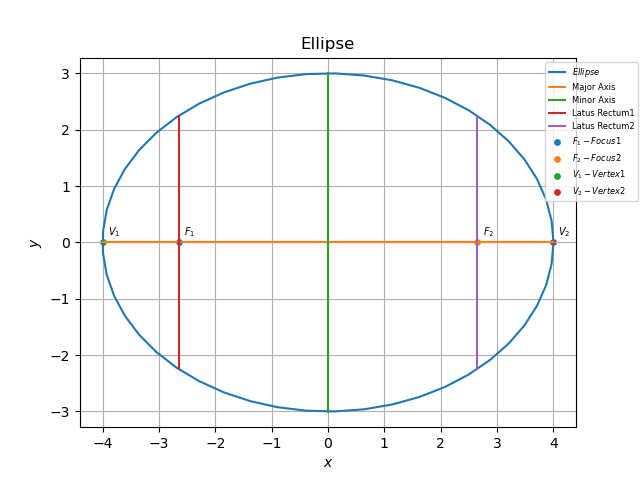
\includegraphics[scale=0.5]{conic.png}    
 \end{center}\vspace{1mm}
 From the figure,\\ \vspace{1mm}
Total area of portion is given by, \\ \vspace{1mm}
Total Area=(area enclosed by the line)-(area of parabola under the line )

\subsection*{Area Under the line}

\begin{align}
\implies A1=\int_{-2}^{4} \frac{3x+12}{2} \,dx
\end{align}
by solving the above equation we get area of triangle \textbf{$45 m^2$}
\subsection*{Area of enclosed ny the parabola under line}

\begin{align} 
\implies A2=\int_{-2}^{4}\frac{3x^2}{4} \,dx 
\end{align}
by solving the above equation we get area of parabola under the line \textbf{$18 m^2$}

the total area is

\vspace{3mm}
$\implies A=63 m^2 $\vspace{3mm}

The area enclosed by the parabola and line is ,
\begin{align}
\hspace{-4.25cm}A= 27 m^2
\end{align}
 \vspace{2mm} \textbf{Construction}
\begin{center}
\setlength{\arrayrulewidth}{0.5mm}
\setlength{\tabcolsep}{6pt}
\renewcommand{\arraystretch}{1.5}
    \begin{tabular}{|l|c|}
    \hline 
    \textbf{Points} & \textbf{coordinates} \\ \hline
   B & $\myvec{
   4\\
   12
   } $ \\\hline
   A & $\myvec{
   -2\\
   3
   } $ \\\hline
      \end{tabular}
  \end{center}
  \end{multicols}
 
Get the python code of the figures from

\begin{table}[h]
\large
\centering
\framebox{
\url{https://github.com/chandana531/cchandana_fwc/blob/main/conic_assignment/code/conic.py}}
\bibliographystyle{ieeetr}
\end{table} 
 
\end{document}
 